\documentclass{article}

\usepackage{booktabs}
\usepackage{tabularx}
\usepackage{graphicx}
\usepackage{hyperref}
\usepackage{enumitem}
\usepackage[capitalise]{cleveref}

\input{../Comments}
\input{../Common}

\title{User Guide\\\progname{} (InfraRAT Web Application)}
\author{\authname}
\date{}

\begin{document}

\begin{table}[hp]
\caption{Revision History} \label{TblRevisionHistory}
\begin{tabularx}{\textwidth}{llX}
\toprule
\textbf{Date} & \textbf{Developer(s)} & \textbf{Change}\\
\midrule
2026-04-05 & Jeremy Orr & Added full user guide content for frontend functionality\\
2026-04-05 & --- & Rewrote guide from frontend source: InfraRAT features, routes, downloads, dashboards\\
\bottomrule
\end{tabularx}
\end{table}

\vspace{0.5em}
\noindent\textit{This document uses date-based revision entries. Add a new row when frontend functionality changes significantly.}

\newpage

\maketitle

\tableofcontents
\newpage

\section{Introduction}
\label{sec:introduction}

The deployed web client is branded \textbf{InfraRAT}. It is a browser-based front end for exploring a large rat behavioural dataset (on the order of twenty thousand trials): natural-language and structured querying, inventory counts and session lists, configurable charts and heatmaps, pre-built comparison dashboards, and per-session trajectory analysis.

This guide describes what appears in the application (\texttt{src/ocd-rat-frontend}) and how end users can accomplish common tasks. The product name in the UI and footer is InfraRAT; \progname{} refers to the capstone project context in \texttt{../Common.tex}.

Note: this file imports macros from \texttt{../Comments} and \texttt{../Common}. Ensure both files are included when distributing the document.

\section{Quick Start}
\label{sec:quick-start}

\begin{enumerate}[nosep]
  \item Open the deployed application URL in your browser.
  \item Read \textbf{Home} for an overview, carousel use cases, and example query wording.
  \item Use \textbf{Query} in \textbf{Ask} mode for conversational answers, or \textbf{Select} mode for generated SQL and tabular results.
  \item Open \textbf{Inventory} (\emph{Data Inventory}) to count sessions and files under filters, optionally list up to 500 sessions, and download file bundles.
  \item Use \textbf{Visualizations} to open bar chart, heatmap, spatial heatmap, velocity profile, or the graph-query dashboard.
  \item Use \textbf{ToolBox} to load one session, inspect tables and plots, and view summary metrics.
  \item Open \textbf{About} (info icon in the header) for team information and FAQs.
\end{enumerate}

\section{Access, Authentication, and Environment}
\label{sec:access}

There is no login or SSO screen in the current front end. Access is via the deployment URL your administrator provides.

When the app is run locally on port 8080, the header may show a \textbf{STAGING} badge next to the product name.

\section{Global Layout}
\label{sec:layout}

\subsection{Header and navigation}
\label{subsec:navigation}

The sticky header shows the InfraRAT logo and name. Primary links (desktop) or a popover menu (narrow screens) include:
\begin{itemize}[nosep]
  \item \textbf{Home} --- \texttt{/}
  \item \textbf{Query} --- \texttt{/query}
  \item \textbf{Visualizations} --- \texttt{/visualizations}
  \item \textbf{Inventory} --- \texttt{/inventory}
  \item \textbf{ToolBox} --- linked from the bar as \texttt{/toolbox} (the registered route in code uses mixed case; if a link fails, try \texttt{/ToolBox} on case-sensitive hosts).
\end{itemize}

To the right, an \textbf{About} control (info icon) opens \texttt{/about}. A GitHub icon links to the project issues page for bug reports and feedback.

\subsection{Footer}
\label{subsec:footer}

The footer shows version text (e.g.\ InfraRAT v1.0), course attribution, and external links to the FRDR repository and the Szechtman lab collection.

\subsection{Missing pages}
\label{subsec:notfound}

Unknown paths render a not-found page.

\section{Home Page}
\label{sec:home}

The home page states the purpose of the platform (data analysis for animal models of OCD) and highlights scale (twenty-thousand-plus trials).

\subsection{Carousel}
\label{subsec:home-carousel}

An auto-advancing carousel summarizes use cases: dataset access and download, visualization and analysis, natural language querying, experiment playback, processing pipeline, and API access. These are orientation slides, not separate routes.

\subsection{Illustrations and examples}
\label{subsec:home-examples}

Still images contrast video trials with temporal or tabular representations. Example natural-language prompts appear with short illustrative copy. A \emph{sample} results table (demo rows such as trial ID, group, checking count, home-base duration, video sync) demonstrates the \emph{shape} of query output; it is not live data from your deployment.

\begin{figure}[ht]
\centering
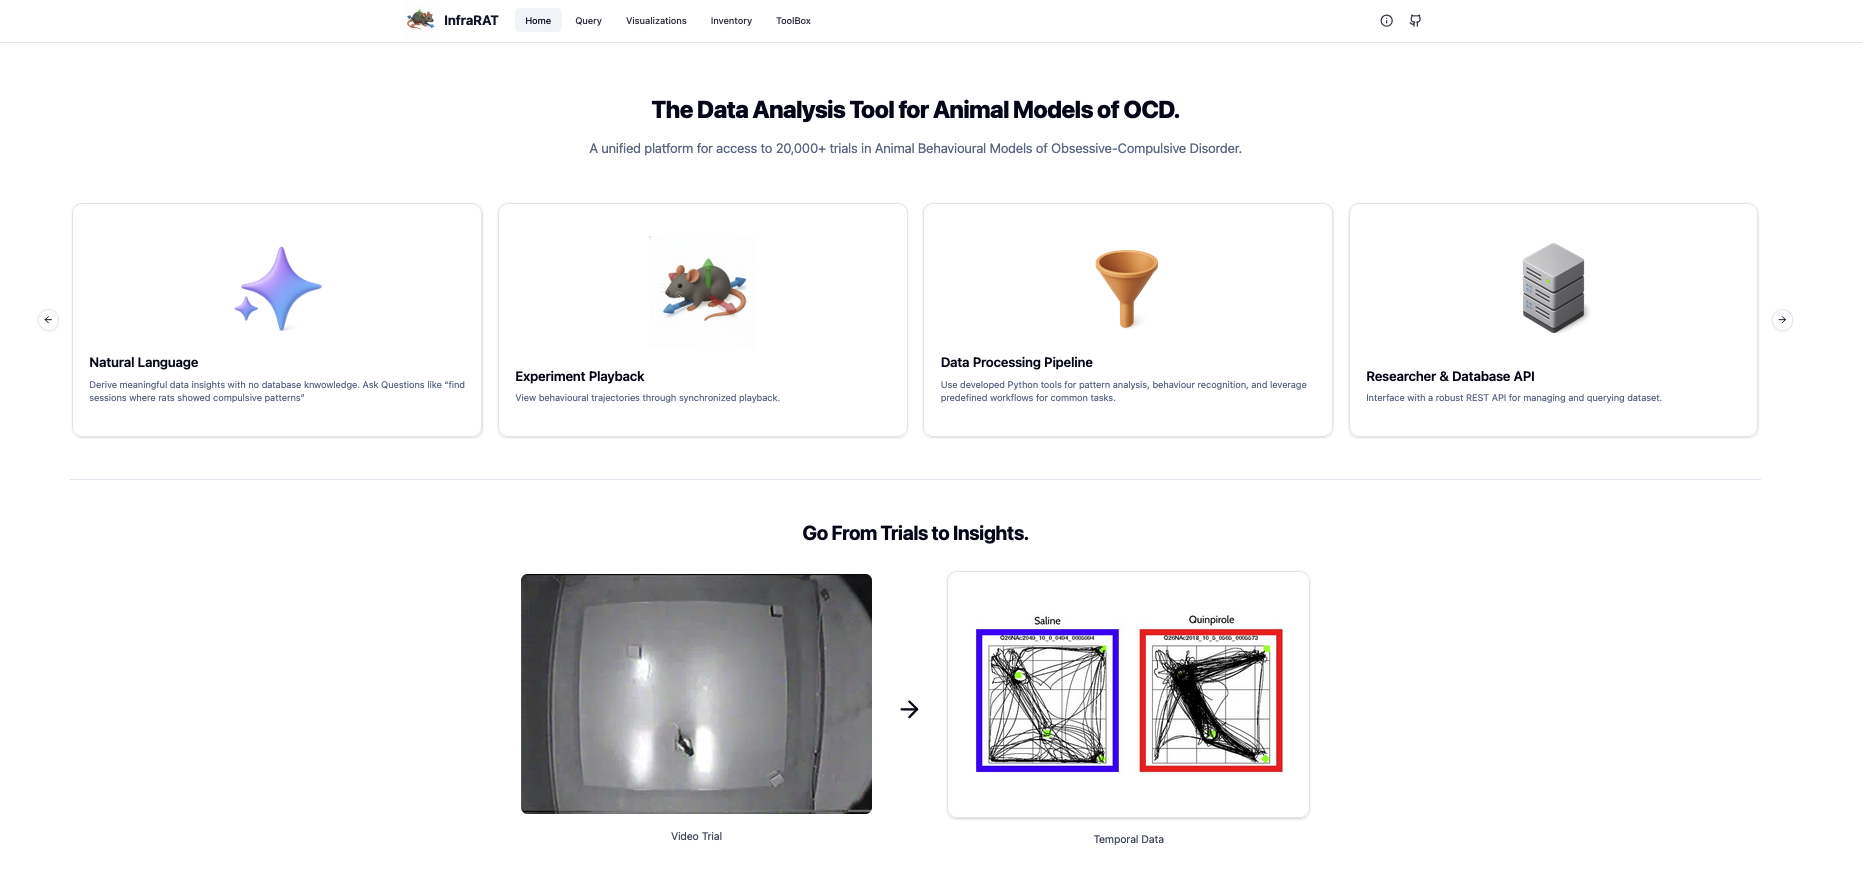
\includegraphics[width=0.95\textwidth]{homepage.png}
\caption{Home page overview: headline, carousel, and example content.}
\label{fig:home}
\end{figure}

\section{About Page}
\label{sec:about}

The About page (\texttt{/about}) lists faculty and student team members and credits the prior capstone cohort. An accordion presents frequently asked questions (purpose of the platform, audience, hosted data types, downloads). A button invites users who need more detail to go to \textbf{Query} and ask there.

\section{Query Page}
\label{sec:query}

The Query page is the main text interface to the dataset. The empty state title is \emph{Query}; the subtitle reads \emph{Talk to the FRDR}.

\subsection{Ask and Select modes}
\label{subsec:query-mode}

A toggle switches between:
\begin{itemize}[nosep]
  \item \textbf{Ask} --- the client streams a natural-language answer from the backend (\texttt{/ask/}). Replies appear as chat bubbles; text wrapped in \texttt{**} pairs is shown in bold.
  \item \textbf{Select} --- the same natural-language input is sent to the NLP SQL endpoint (\texttt{/nlp/}). The response is rendered as a structured card: \emph{Query Plan} (rationale), \emph{SQL Query} (monospace), and \emph{Results}. The inline results table shows at most fifty rows with a note if more exist.
\end{itemize}

User messages appear on the right (dark bubble); assistant content on the left (light bubble or SQL card).

\subsection{Sending a message}
\label{subsec:entering-queries}

Use the bottom text area (placeholder: ``Ask, Search or Chat\ldots''). Press Enter to send; use Shift+Enter if you need a newline. A send button is also available.

Example prompts shown on Home include natural-language questions and a trial-specific request for \texttt{(x,y,t)} trajectory data.

\subsection{Session table after Select}
\label{subsec:query-results}

After a successful \textbf{Select} response, a \textbf{Sessions} card below the chat lists the full result set with a horizontal scrollable table and a result count.

\begin{figure}[ht]
\centering
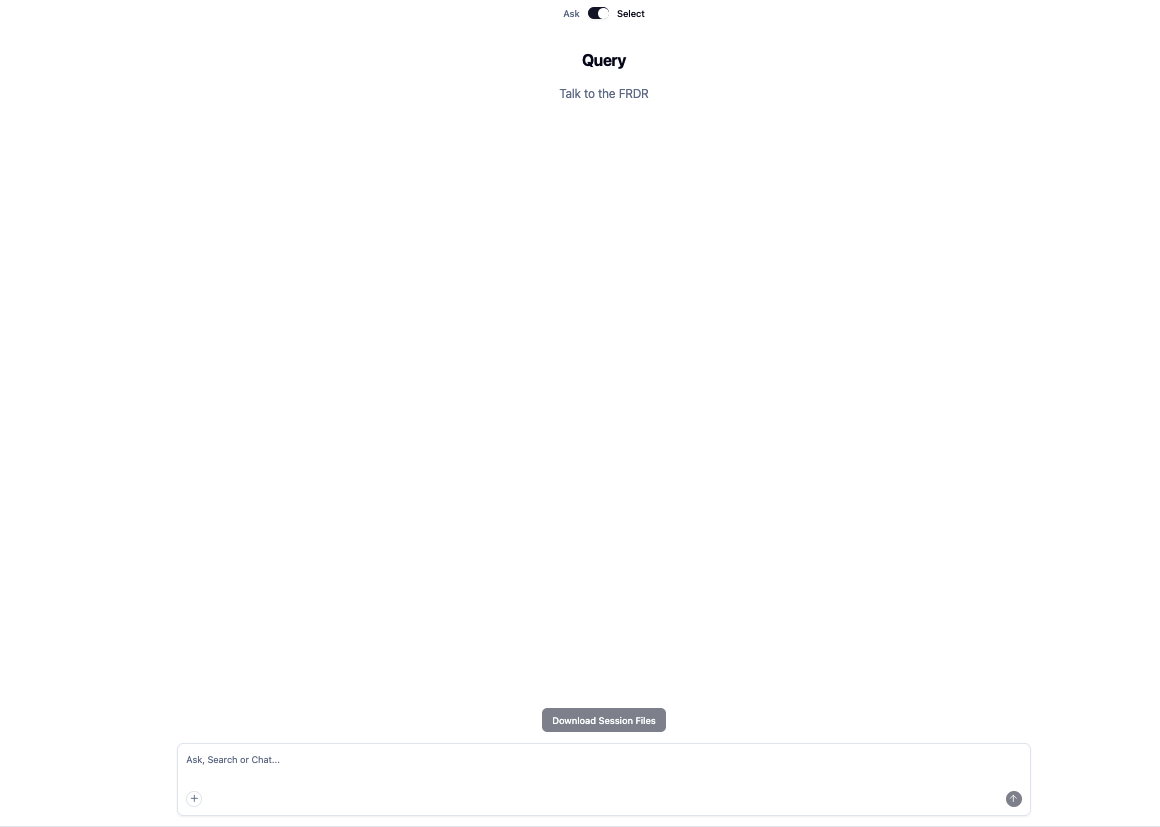
\includegraphics[width=0.95\textwidth]{QueryPage.png}
\caption{Query page: mode toggle, chat or SQL result, session summary table.}
\label{fig:query}
\end{figure}

\subsection{Downloading session files (Query)}
\label{subsec:download-files}

\textbf{Download Session Files} is enabled only when the \emph{last} message in the thread is a \textbf{Select} SQL result (not after a pure \textbf{Ask} reply). Opening it shows checkboxes for \textbf{CSV}, \textbf{EWB}, \textbf{GIF}, \textbf{JPG}, and \textbf{MPG}. Confirming starts a job; a progress bar reports completion until the browser downloads a ZIP named \texttt{FRDR\_FILES\_<job-id>.zip}. The archive is built for the sessions returned by your last Select query.

\section{Data Inventory (Inventory Page)}
\label{sec:inventory}

The page title is \textbf{Data Inventory}. It explains that counts are by raw data type (video, track files, and similar) and that filters narrow which sessions are included.

\subsection{Quick presets}
\label{subsec:inventory-presets}

Two buttons apply common scopes without configuring the sidebar:
\begin{itemize}[nosep]
  \item \textbf{Show full inventory} --- all sessions (clears manual filter state for the preset request).
  \item \textbf{Unoperated rats only} --- restricts to surgery type \emph{Unoperated}.
\end{itemize}

\subsection{Filters (sidebar)}
\label{subsec:inventory-filters}

Filters are grouped in accordions:
\begin{itemize}[nosep]
  \item \textbf{Drug treatment} --- multi-select checkboxes; multiple drugs combine (OR semantics as implemented by the API request body).
  \item \textbf{File types} --- multi-select by object type (e.g.\ video vs track files).
  \item \textbf{Drug Regiments} --- multi-select for fine-grained prescription or regimen labels (the UI label uses this spelling).
  \item \textbf{Brain manipulation} --- dropdowns for surgery type and brain region.
  \item \textbf{Apparatus} --- apparatus, pattern, and testing room.
  \item \textbf{Session type} --- single select.
\end{itemize}

Use \textbf{Apply} to fetch counts; \textbf{Clear} resets selections and clears results and the session table.

\subsection{Results area}
\label{subsec:inventory-results}

After Apply (or a preset), the main column shows:
\begin{itemize}[nosep]
  \item a card for \textbf{sessions matching filters} (with an info tooltip defining a session as one behavioural trial),
  \item per-type cards with file counts and session counts (tooltips clarify video vs track where applicable),
  \item a \textbf{Counts by data type} bar chart.
\end{itemize}

\textbf{View sessions (up to 500)} loads a scrollable table of matching sessions (column set from the API). Errors appear in a highlighted banner.

\subsection{Downloading session files (Inventory)}
\label{subsec:inventory-download}

\textbf{Download Session Files} in the sidebar is enabled when a session list is loaded and non-empty. The same ZIP and format checkboxes apply as on Query, but the backend uses filter-based session selection rather than the last NLP query.

\section{Visualizations Hub}
\label{sec:visualizations-hub}

The hub (\texttt{/visualizations}) lists tiles with short descriptions and an \textbf{Open} control:
\begin{itemize}[nosep]
  \item \textbf{Bar Chart} --- \texttt{/visualizations/bar-chart}
  \item \textbf{Heatmap} --- \texttt{/visualizations/heatmap}
  \item \textbf{Spatial Heatmap} --- \texttt{/visualizations/spatial-heatmap}
  \item \textbf{Velocity Profile} --- \texttt{/visualizations/velocity-profile}
  \item \textbf{Query Visualizations} --- \texttt{/visualizations/graph-query-dashboard}
\end{itemize}

There is no tile for the line chart on this hub, but the application still registers \texttt{/visualizations/line-chart} (see \cref{subsec:line-chart}).

\begin{figure}[ht]
\centering
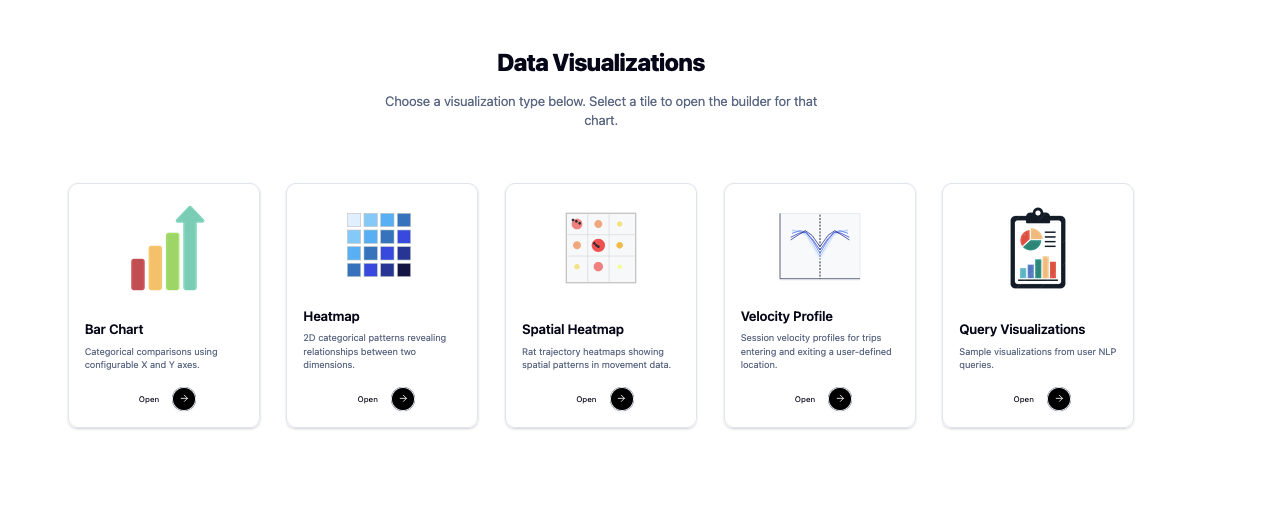
\includegraphics[width=0.95\textwidth]{Visualizations.png}
\caption{Visualizations hub: tiles linking to each builder or dashboard.}
\label{fig:visualizations}
\end{figure}

\subsection{Bar chart builder}
\label{subsec:bar-chart}

The bar chart page loads options from \texttt{/visualizations/available}. Choose an \textbf{X-Axis (Group By)} and a \textbf{Y-Axis} metric; the chart requests \texttt{/visualizations/barchart} with the chosen axes. Axis labels and units come from the API.

\subsection{Line chart builder}
\label{subsec:line-chart}

The line chart page uses the same options endpoint with \textbf{X-Axis (Time Period)} and a \textbf{Y-Axis} metric appropriate for trends over time. Data is loaded from the line-chart endpoint exposed by the visualization API.

\subsection{Heatmap builder}
\label{subsec:heatmap}

Select two categorical dimensions (X and Y) and a \textbf{metric} for cell colour intensity. The client fetches heatmap-specific axes and metrics from \texttt{/visualizations/available}, then requests aggregated heatmap data from the backend.

\subsection{Spatial heatmap}
\label{subsec:spatial-heatmap}

This tool builds an occupancy-style map from trajectory points for one or more sessions:
\begin{itemize}[nosep]
  \item \textbf{Sessions} --- scrollable checklist loaded from the same session list source as ToolBox; \textbf{Clear All} deselects. Sessions without trajectory data are reported as unsupported.
  \item \textbf{Bin size (cm)} --- discrete choices (e.g.\ 1, 2, 4, 5, 8, 10, 16, 20, 32, 40, 80, 160) on a 160\,cm arena grid.
  \item \textbf{Metric} --- \emph{Entries (Visits)} (bin entry counts) or \emph{Time Spent} (dwell time between samples).
  \item \textbf{Fixed scale max (optional)} --- caps the colour scale so multiple sessions stack visibly on the same scale.
  \item \textbf{Home base} --- enter four corners (top-left, top-right, bottom-left, bottom-right) in cm, then \textbf{Set Home Base}; optional \textbf{Clear}. When set, the UI shows time-in-home-base as a fraction of total session time. Fixed arena objects are drawn for reference.
  \item \textbf{Export Data to CSV} and \textbf{Export Map to PNG} --- download bin-level data or a rendered canvas image.
\end{itemize}

Hovering the map shows bin coordinates, metric value, and contributing session IDs.

\subsection{Velocity profile}
\label{subsec:velocity-profile}

Steps:
\begin{enumerate}[nosep]
  \item \textbf{Select session} --- searchable dropdown (same session search endpoint as ToolBox).
  \item \textbf{Define zone} --- centre \texttt{X}, \texttt{Y}, and \texttt{Radius} in tracking units (coordinates can be cross-checked in ToolBox).
  \item \textbf{Parameters} --- \emph{Max frames per side} (allowed range 10--500, default 150) and \emph{Min trip frames} (shorter segments are treated as lingering and excluded).
  \item \textbf{Colouring} --- \emph{Temporal gradient} (each trip coloured along time) or \emph{Time-slice highlight} (grey baseline with a slider to emphasize a trip index range).
  \item \textbf{Generate} --- fetches entering and exiting velocity segments and plots them. Summary tiles show total trips, segment counts, and session frames. If no trips qualify, the UI suggests increasing radius or lowering the minimum trip length.
\end{enumerate}

\subsection{Query Visualizations (graph-query dashboard)}
\label{subsec:graph-dashboard}

This page loads pre-defined multi-panel layouts backed by \texttt{/toolbox/graph-query/<id>/}. A \textbf{Graph Set} dropdown switches between:
\begin{itemize}[nosep]
  \item \textbf{Query Visualization 1: Tucci et al.\ (2014) format} --- snapshot-style bar panels at selected injections with error bars, plus a legend card. Panels include frequency of checking, length of check, recurrence time, stops before returning, and duration of rest.
  \item \textbf{Query Visualization 2: Ballester et al.\ (2015) format} --- line charts across injections 1--10 for the same behavioural measures, with cohort markers and error bars.
\end{itemize}

Each set shows a long methodological description on the page (filters, comparisons, and literature context). If some panels fail to load, a warning appears while successful panels still render. Tooltips on charts show mean, SEM, and $n$ where available.

\section{Analysis ToolBox}
\label{sec:toolbox}

The ToolBox page title is \textbf{Analysis Toolbox}. It focuses on a single session at a time.

\subsection{Session search and load}
\label{subsec:toolbox-selection}

Type in the \emph{Search or select a session\ldots} field; the client queries the backend for matching session IDs and shows a dropdown. Choose an ID and click \textbf{Load Session}. While loading, the button is disabled and a short loading indicator may appear.

\subsection{Successful load}
\label{subsec:toolbox-loading}

On success, the layout includes:
\begin{itemize}[nosep]
  \item \textbf{Session Info} --- metadata table (columns depend on API).
  \item \textbf{Data Points} --- scrollable trajectory or frame table (e.g.\ position and time columns).
  \item A \textbf{static image} preview when the API returns image bytes.
  \item \textbf{PathPlot} --- an interactive trajectory plot built from the same points.
\end{itemize}

\subsection{Metrics cards}
\label{subsec:toolbox-metrics}

Three cards summarize:
\begin{itemize}[nosep]
  \item \textbf{Distance Travelled} (metres) --- if the value is \texttt{N/A}, a \textbf{Generate Distance?} button recomputes distance using legacy session and trial identifiers from session info.
  \item \textbf{Total Number of Checks}.
  \item \textbf{Average Check Time}, labelled in \emph{log(10) seconds} in the UI.
\end{itemize}

\subsection{Unsupported session}
\label{subsec:toolbox-unsupported}

If the backend reports failure for the chosen ID, a message states that the session is not supported.

\begin{figure}[ht]
\centering
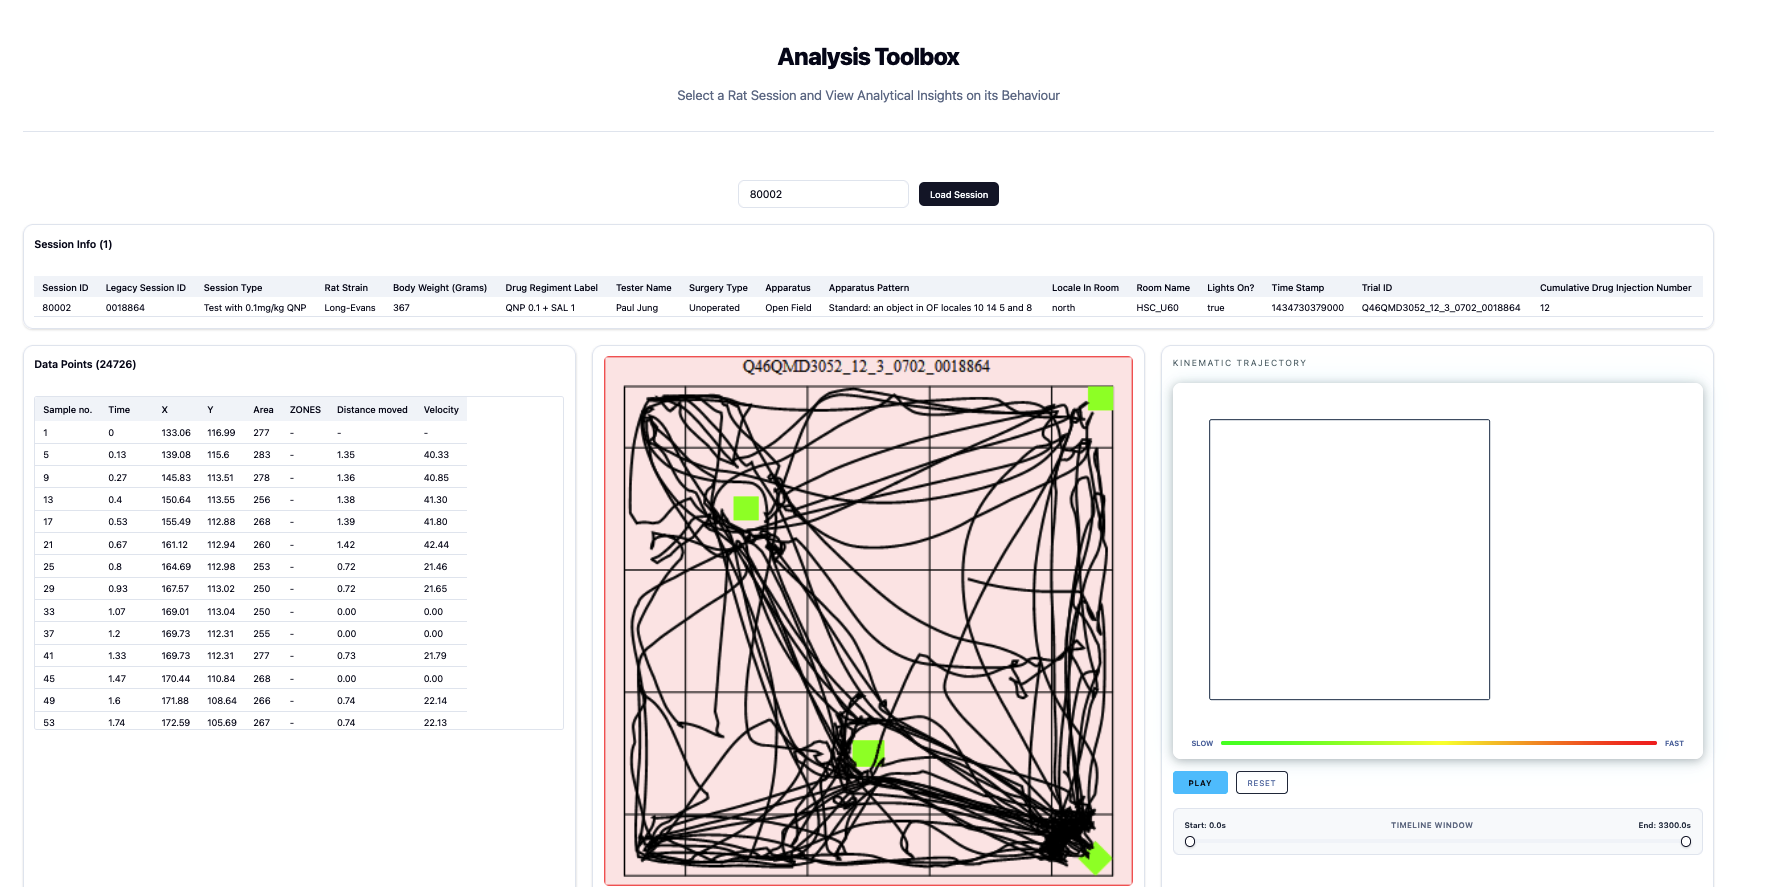
\includegraphics[width=0.95\textwidth]{ToolBoxPage.png}
\caption{ToolBox: session selection, tables, trajectory plot, and metrics.}
\label{fig:toolbox}
\end{figure}

\section{Downloads and File Formats}
\label{sec:file-format}

Bulk downloads from Query (after Select) and Inventory (after loading sessions) produce a single ZIP archive named \texttt{FRDR\_FILES\_<job-id>.zip}. Inside, the server includes only the extensions you selected:

\begin{description}[nosep]
  \item[CSV] Tabular exports for spreadsheets and analysis.
  \item[EWB] Experimental workflow / behavioural files used in the research pipeline.
  \item[JPG] Still images.
  \item[MPG] Video recordings.
  \item[GIF] Short animated summaries.
\end{description}

Spatial heatmap exports are separate browser downloads (CSV of bins, PNG of the canvas) and do not use the FRDR ZIP flow.

\section{Glossary}
\label{sec:glossary}

\begin{description}[nosep]
  \item[Ask mode] conversational answers streamed from the ask endpoint (no SQL card).
  \item[FRDR] Federated Research Data Repository; referenced in copy and download naming.
  \item[Select mode] natural language interpreted into SQL with tabular results and optional ZIP download.
  \item[Session] one behavioural experimental trial for a subject (definition also in Inventory tooltips).
  \item[Graph set] a predefined dashboard layout and backing queries on the Query Visualizations page.
  \item[Home base] user-defined polygon on the spatial heatmap used for dwell-time ratio.
\end{description}

\section{Troubleshooting}
\label{sec:troubleshooting}

\begin{itemize}[nosep]
  \item If \textbf{Download Session Files} stays disabled on Query, run a \textbf{Select} query that returns rows so the last message is a SQL result; Ask-mode threads do not enable the button.
  \item On Inventory, run \textbf{View sessions (up to 500)} before download if the sidebar button remains disabled.
  \item If the ToolBox link 404s, try \texttt{/ToolBox} vs \texttt{/toolbox} depending on server case sensitivity.
  \item Refresh the page on transient network errors; wait for ZIP jobs to finish before starting another.
  \item For platform issues, use the GitHub issues link in the header or contact your deployment administrator.
\end{itemize}

\end{document}
